\section{Situación Actual}

En la actualidad podemos encontrar diversos intentos de modernizar los procesos administrativos de entidades públicas y podemos tomar sus experiencias como inspiración para la realización de una herramienta reutilizable de software. Además, existen paquetes de software que, aunque de manera indirecta, pueden ayudar en la creación de trámites.
\subsection{Normativa relevante}
\subsubsection{Gobierno Electrónico y su normativa}
Cuando hablamos de Gobierno Electrónico y su normativa es menester citar a la Constitución Política del Estado Plurinacional de Bolivia, misma que en su Art. 103 y 298 denota la importancia del desarrollo de la ciencia y la investigación a favor de las bolivianas y los bolivianos. Además, reconoce como prioridad el uso de las tecnologías y comunicación para el vivir bien. Al respecto el Artículo 103 establece lo siguiente:"I. El Estado garantizará el desarrollo de la ciencia y la investigación científica, técnica y tecnológica en beneficio del interés general. Se destinarán los recursos necesarios y se creará el sistema estatal de ciencia y tecnología. II. El Estado asumirá como política la implementación de estrategias para incorporar el conocimiento y aplicación de nuevas tecnologías de información y comunicación. III. El Estado, las universidades, las empresas productivas y de servicio públicas y privadas, y las naciones y pueblos indígena originario campesinos, desarrollarán y coordinarán procesos de investigación, innovación, promoción, divulgación, aplicación y transferencia de ciencia y tecnología para fortalecer la base productiva e impulsar el desarrollo integral de la sociedad, de acuerdo con la ley." Asimismo el Artículo 298 de la citada normativa legal en su parte pertinente establece lo siguiente: "(...)II. Declara prioridad nacional la promoción del uso de las tecnologías de información y comunicación para procurar el vivir bien de todas las bolivianos y bolivianos. (...)"
A su vez es menester citar la Ley N°164 - Ley General de Comunicaciones, Tecnologías de Información y Comunicación, misma que en su Artículo 71 declara prioridad nacional la promoción y uso de tecnologías de información y comunicación para procurar el vivir bien de todas las bolivianas y bolivianos. Por otra parte, el párrafo I del el Artículo 72 de la citada noma legal, establece el rol de Estado con referencia al uso de las TIC´S, el despliegue y uso de infraestructura, el desarrollo de contenidos y aplicaciones, la protección de las usuarias y usuarios, la seguridad informática y redes como mecanismos de democratización de oportunidades para todos los sectores de la sociedad y especialmente para aquellos con menores ingresos y con necesidades especiales, a su vez el Artículo 75 de la citada norma legal, hace referencia a Gobierno Electrónico, mismo que establece de forma expresa lo siguiente: "I. El nivel central del Estado promueve la incorporación del Gobierno Electrónico a los procedimientos gubernamentales, a la prestación de sus servicios y a la difusión de información, mediante una estrategia enfocada al servicio de la población. II. El Órgano Ejecutivo del nivel central del Estado, elaborará los lineamientos para la incorporación del Gobierno Electrónico." Asimismo el Artículo 76, define el Alcance de Gobierno Electrónico, mismo que señala lo siguiente: "(...) El Estado fijará los mecanismos y condiciones que las entidades públicas aplicarán para garantizar el máximo aprovechamiento de las tecnologías de la información y comunicación, que permitan lograr la prestación de servicios eficientes." 
 Otra normativa que regula lo referente al Gobierno Electrónico, se puede citar al Reglamento para el Desarrollo de Tecnologías de Información y Comunicación - Decreto Supremo N° 1793, mismo que en su Art. 17 establece el objetivo de Gobierno Electrónico, señalando lo siguiente: "(...)I. Modernizar y transparentar la gestión pública, otorgando servicios y atención de calidad a la ciudadanía, garantizando el derecho a la información, así como contribuir a la eficiencia y eficacia de los actos administrativos en los procesos internos del gobierno, mediante el uso de las tecnologías de información y comunicación y otras herramientas. II. Generar mecanismos tecnológicos de participación y control social, mediante el uso de TIC por parte de los ciudadanos, organizaciones sociales y pueblos y naciones indígena originario campesinos."
\subsubsection{Software Libre y su regulacioón normativa}
El art. 77 de la Ley de Telecomunicaciones establece lo siguiente: “ARTICULO 1 (SOFTWARE LIBRE) I. Los Órganos Ejecutivo, Legislativo, Judicial y Electoral en todos sus niveles, promoverán y priorizarán la utilización del software libre y estándares abiertos, en el marco de la soberanía y seguridad nacional. II. El Órgano Ejecutivo del nivel central del Estado, elaborara el plan de implementación de software libre y estándares abiertos en coordinación con los demás órganos del Estado y entidades de la administración pública.”
Cuando se habla de Software libre y su normativa, se puede citar al Reglamento para el Desarrollo de Tecnologías de Información y Comunicación – Decreto Supremo N°1793, mismo que en su parte pertinente establece lo siguiente: Articulo 3.- DEFINICIONES. Además de las definiciones técnicas establecidas en la Ley N°164, para el cumplimiento del presente reglamento se adoptan las siguientes definiciones: (…) II. Respecto a software libre. 
a. Programa o software: Cualquier secuencia de instrucciones finita usada por un dispositivo de procesamiento digital de datos para llevar a cabo una tarea específica o resolver un problema determinado, incluyendo todas las dependencias necesarias para su pleno funcionamiento; 
b. Código fuente o programa fuente: Conjunto completo de instrucciones y archivos digitales originales, legible para el ser humano, tal y como fue escrito por el programador, en un lenguaje de programación específico, más todos los archivos digitales de soporte, como tablas de datos, imágenes, especificaciones, documentación y todo otro elemento que sea necesario para producir el programa ejecutable a partir de ellos; 
c. Software libre: Software licenciado por su autor, bajo una licencia de código fuente abierta, de manera tal que permita al usuario el ejercicio de las siguientes libertades:
• Ejecutar el software, para cualquier propósito, sin restricción alguna; 
• Estudiar cómo funciona el software y modificarlo para que cumpla un determinado propósito, a través del acceso al código fuente del mismo y todos los componentes que hacen posible su funcionamiento. El acceso al código fuente es una condición necesaria e imprescindible; 
• Redistribuir copias del software; 
• Distribuir copias de las versiones modificadas a terceros. El acceso al código fuente es una condición necesaria e imprescindible. 
d. Software propietario o software privativo: Todo software que no cumpla parcial o totalmente con cualquiera de las condiciones mencionadas para el software libre, se considera para los efectos del presente Reglamento, software propietario; 
e. Estándar abierto: Es una especificación técnica o protocolo normalizado: 
• Cuyas especificaciones técnicas, completas y coherentes, están sujetas a una evaluación pública completa, se puede usar sin restricciones y está disponible por igual para todos los usuarios y/o partes, sin costo alguno para su uso; 
• Que no necesita ningún componente o extensión adicional que tenga dependencias con formatos o protocolos que no cumplan la definición de Estándar Abierto; 
• Que está libre de cláusulas legales o técnicas que limiten o restrinjan su utilización por cualquier usuario y/o parte o en cualquier modelo de negocio;
 • Que es gestionado y puede ser desarrollado independientemente por cualquier organización en un proceso abierto a la participación equitativa e inclusiva de competidores, usuarios, especialistas del área de aplicación y terceras partes;
 • Que esté disponible en al menos una implementación completa, cuya documentación y especificación técnica está disponible para todas las partes con grado de detalles suficientes para un desarrollo correcto y de calidad. 
f. Repositorio estatal de software libre: Es el sistema informático que contiene los sistemas y aplicaciones libres desarrollados por o para el Estado, de manera directa o a través de terceros.”
Asimismo, el Art. 4 del mismo reglamento establece lo siguiente: “Articulo 4.- (PRINCIPIOS) (…) IV. Software: El software a ser utilizado por las entidades públicas debe regirse por los siguientes principios: a. Soberanía tecnológica: Debe permitir al Estado Plurinacional de Bolivia ejercer pleno control sobre las aplicaciones informáticas o software que utiliza, asegurando la independencia tecnológica del país y la seguridad informática del Estado; b. Seguridad informática del código fuente: Debe permitir al Estado Plurinacional de Bolivia la posibilidad de auditar, conocer y modificar el código fuente del mismo sin requerir ningún tipo de autorización, para obtener el comportamiento deseado de parte de ellas y ningún otro no consentido o requerido, precautelando la seguridad, independencia y soberanía tecnológica de Bolivia; c. Descolonización del conocimiento tecnológico: Debe permitir al Estado Plurinacional de Bolivia romper los lazos de dependencia tecnológica e informacional con respecto a terceros, garantizando la soberanía tecnológica y seguridad informática; y avanzar en el proceso de desarrollo de capacidades científicas e institucionales que permitan el desarrollo de la economía nacional en la construcción del vivir bien. (…)”
De igual forma el art. 19 de la citada norma legal, establece lo siguiente: “Articulo 19.- (PLAN DE IMPLEMENTACIÓN DE SOFTWARE LIBRE Y ESTÁNDARES ABIERTOS). I. El Ministerio de Planificación del Desarrollo en coordinación con el Ministerio de Obras Públicas, Servicios y Vivienda, a través del Viceministerio de Telecomunicaciones y la ADSIB, es la instancia responsable de elaborar, promover, gestionar y articular el Plan de Implementación de Software Libre y Estándares Abiertos para los Órganos Ejecutivo, Legislativo, Judicial y Electoral en todos sus niveles del Estado Plurinacional de Bolivia, así como de su permanente actualización. II. El Plan de Implementación de Software Libre y Estándares Abiertos establecerá los mecanismos para el desarrollo comunitario de aplicaciones de Software Libre, transversales a las necesidades del Estado Plurinacional. III. La ejecución del Plan de Implementación de Software Libre y Estándares Abiertos, estará a cargo de las entidades públicas. IV. El seguimiento a la ejecución del Plan de Implementación de Software Libre y Estándares Abiertos estará a cargo de la ADSIB en coordinación con cada entidad de la administración pública del Estado.” De igual manera en su Art. 20 se establece lo siguiente: “ARTÍCULO 20.- (OBJETIVO DEL PLAN). Establecer las condiciones y mecanismos para la implementación, uso, estudio, auditoria, investigación y desarrollo de software libre y estándares abiertos en las entidades públicas.”  De igual manera en su artículo 21 establece: “ARTÍCULO 21.- (LINEAMIENTOS DEL PLAN). El Plan de Implementación de Software Libre y Estándares Abiertos, debe considerar mínimamente los siguientes lineamientos: a. Posibilitar la implementación, uso y desarrollo de Software Libre y Estándares Abiertos en las plataformas informáticas, aplicaciones, ordenadores, redes informáticas, intercambio de datos y publicación de contenidos digitales de los órganos del Estado Plurinacional de Bolivia; b. Promover el avance del proceso de descolonización del conocimiento; c. Promover la formación, especialización y capacitación de recursos humanos en software libre y estándares abiertos en coordinación con los órganos del Estado y entidades de la administración pública; d. Promover mecanismos de cooperación internacional en materia de software libre y estándares abiertos, en respeto de la soberanía y seguridad informática del Estado Plurinacional de Bolivia; e. Establecer los mecanismos de seguimiento y control que garanticen la aplicación del presente Reglamento y el Plan de Implementación de Software Libre y Estándares Abiertos; f. Promover el desarrollo de software libre en los sectores público y privado, favoreciendo a los profesionales y empresas bolivianas; g. Establecer las condiciones y jerarquización para fortalecer las unidades de sistemas de las entidades públicas, de modo que puedan cumplir con los objetivos del Reglamento.” 
\subsubsection{Soberania Digital y las leyes}
Al respecto es menester tener en cuenta lo estipulado en el Artículo 1 de la Constitución Política del Estado que establece lo siguiente: “(…) Bolivia se constituye en un Estado Unitario Social de Derecho Plurinacional Comunitario, libre, independiente, soberano, democrático, intercultural, descentralizado y con autonomías. (…)” asimismo el articulo 7 de la citada norma legal establece: “Articulo 7.- (…) La soberanía reside en el pueblo boliviano se ejerce de forma directa y delegada. De ella emanan, por delegación, las funciones y atribuciones de los órganos del poder público, es inalienable e imprescriptible.” A su vez el art. 103 de la carta magna de nuestro país establece: Artículo 103.- (…) III. El estado, las universidades, las empresas productivas y de servicio públicas y privadas, y las naciones y pueblos indígenas originario, campesinos, desarrollan y coordinaran procesos de investigaciones, innovación, promoción, divulgación, aplicación y transferencia de ciencia y tecnología para fortalecer la base productiva e impulsar el desarrollo integral de la sociedad de acuerdo con ley.
Asimismo, al hablar de soberanía digital y la normativa que regula lo referente a ella, es menester cita a la Ley de Telecomunicaciones, misma que en su Artículo 2 numeral 5 establece lo siguiente: “Articulo 2.- La presente Ley tiene por objetivos: (…) 5. Promover el uso de las tecnologías de información y comunicación para mejorar las condiciones de vida de las bolivianas y bolivianos.” De igual formal el art. 5, numerales 1, 6 y 7 de la citada normativa legal establece: “Articulo 5.- (Principios). El sector de telecomunicaciones y tecnologías de información y comunicación y del servicio postal se regirá bajo los siguientes principios: 1. Acceso universal. El Estado, en todos sus niveles de gobierno, promoverá el derecho al acceso universal a las telecomunicaciones y tecnologías de información y comunicación, así como el servicio postal, para todas y todos los habitantes del Estado Plurinacional de Bolivia, en ejercicio de sus derechos, relacionados principalmente a la comunicación, la educación, el acceso al conocimiento, la ciencia, la tecnología y la cultura. (…) 6. Innovación tecnológica. El estado promoverá el desarrollo de tecnología propia en el aérea de las telecomunicaciones y tecnologías de información y comunicación. (…) 7. Neutralidad tecnológica. El estado fomentara la libre adopción de tecnologías, en el marco de la soberanía nacional y teniendo en cuenta recomendaciones, conceptos y normativas de organismos internacionales competentes e idóneos en la materia. (…)”
Reglamento para el Desarrollo de Tecnologías de Información y Comunicación – Decreto Supremo N°1793, mismo que en su parte pertinente establece lo siguiente: Articulo 3.- DEFINICIONES (…) VII. Respecto a la soberanía. a. Dependencia tecnológica: Es la condición a que someten a los usuarios, sean estos personas, naturales o jurídicas, estados o naciones, las compañías, empresas, naciones o estados que desarrollan, distribuyen o venden tecnología, al negar el acceso al conocimiento de los contenidos, procedimientos, técnicas y procesos necesarios para el uso, desarrollo y distribución de las mismas, a través de licencias, patentes, restricciones prácticas, restricciones legales y otros; de modo que los usuarios vean restringida la posibilidad de controlar, auditar, usar, modificar o desarrollar dicha tecnología; b. Soberanía tecnológica: Es la posesión del control por parte de una nación y/o estado sobre la tecnología que utiliza. Se caracteriza por el acceso al conocimiento sobre el contenido y los procedimientos, procesos y técnicas necesarios para el desarrollo y uso de dicha tecnología, el mismo que le permite auditar, mejorar, desarrollar, modificar y ajustar a sus necesidades específicas la misma, sin la intervención ni autorización específica de terceros; de modo que se garantice la total independencia en cuanto al control de la tecnología utilizada por dicha nación o estado con respecto a compañías, empresas, personas, naciones o estados; c. Descolonización del conocimiento tecnológico e informacional: Es el proceso social y científico que permite romper los lazos de dependencia tecnológica e informacional de una nación y/o estado con respecto a terceras personas, empresas, naciones o estados y desarrollar conocimiento y tecnología propia, acorde a sus necesidades, retos y características, partiendo del diálogo entre los conocimientos locales y universales disponibles. Es un proceso de intercambio cultural, de conocimientos y tecnologías, con otras sociedades, naciones y/o estados dispuestos a compartir sus propios desarrollos e interiorizar los externos, respetando el derecho de los otros a conocer los contenidos y los procedimientos, procesos y técnicas necesarios para el desarrollo y uso de las tecnologías en general y de las tecnologías de la información y la comunicación en particular. La descolonización del conocimiento tecnológico e informacional está directamente relacionada con el desarrollo de capacidades científicas e institucionales para garantizar el manejo y aprovechamiento soberano de los recursos naturales y el desarrollo económico del Estado Plurinacional de Bolivia en la construcción del vivir bien. (…)
\subsubsection{El trámite administrativo y su regulación normativa}
Al respecto cuando hablamos de la regulación normativa del tramite administrativo es menester citar al Decreto Supremo N°3525, el cual en su art. 12 establece lo siguiente:"Artículo 12°.- (Trámites administrativos) I. Las instituciones públicas deberán priorizar en todos sus trámites el uso de tecnologías de información y comunicación a efecto de digitalizar, automatizar, interoperar y simplificar la tramitación de los asuntos que son de su competencia. II. Para facilitar la realización de trámites a la ciudadanía, las entidades públicas, en observancia de su normativa específica, deberán intercambiar entre ellas datos e información mediante interoperabilidad. Los mecanismos y condiciones de publicación y acceso a los servicios de interoperabilidad serán establecidos por el Ente Rector de Gobierno Electrónico y Tecnologías de Información y Comunicación. III. El intercambio de datos e información mediante interoperabilidad no afectará la percepción de recursos de las entidades públicas titulares de la información por la prestación del servicio público. IV. Las entidades públicas no podrán exigir al administrado como requisito ningún documento que hubiera sido emitido por la misma entidad, o cuya información esté disponible mediante servicios de interoperabilidad de otra entidad. V. Las entidades públicas no podrán exigir al administrado como requisito ningún documento que hubiera sido requerido con anterioridad, salvo actualización o modificación y conforme a normativa legal vigente. VI. Las entidades públicas tendrán un plazo máximo de veinte (20) días hábiles a partir de la publicación de un nuevo servicio de interoperabilidad para adecuar sus procesos y procedimientos al mismo" A su vez el Art. 13 del citado decreto establece lo siguiente: "Artículo 13°.- (Entidades generadoras de información) I. Las entidades que conforme a sus atribuciones recolectan, generan, transforman y validan datos o información, son responsables en observancia de su normativa legal específica, de publicar la información y datos como fuente primaria a través de la plataforma de interoperabilidad establecida en el Plan de Implementación de Gobierno Electrónico aprobado mediante el Decreto Supremo Nº 3251, de 12 de julio de 2017. II. En el marco de procesos de actualización, certificación o emisión de copias legalizadas de documentos que aún se encuentren en formato físico, los datos e información pertinente consignados en los mismos deberán ser registrados en medios digitales que permitan ser publicados mediante servicios de interoperabilidad.(...)"
\subsection{Sistemas realizados para el control de trámites}

Sólo en Latinoamérica, cada país reportó mediante las autoridades de gobierno electrónico tener entre 1000 y 5000 trámites diferentes. Esto implica que ya hubo muchos esfuerzos para crear sistemas que digitalicen esta actividad. A continuación se listan algunos.

\subsubsection{A nivel académico}

Podemos encontrar una gran cantidad de proyectos de grado realizados en la región que tratan sobre la implementación de sistemas de control de trámites:

\begin{itemize}
    \item SISTEMA DE CONTROL DE TRÁMITES UTILIZANDO MAQUINAS DE TURING CASO: DIVISIÓN DE GESTIONES ADMISIONES Y REGISTROS U.M.S.A.
    \item Desarrollo e Implementación del Sistema de Tramite
          Documentario en la Municipalidad Provincial de
          Huancayo para la atencion de expedientes.
    \item DESARROLLO DE UN SISTEMA WEB PARA MEJORAR  EL PROCESO DE TRÁMITE DOCUMENTARIO ADMINISTRATIVO DEL HOSPITAL SUB REGIONAL DE  ANDAHUAYLAS
    \item Sistema de información de trámite documentario basado en tecnología web para institutos de educación superior tecnológicos de la región Ancash en el año 2016
    \item Programa de automatización de los procedimientos de trámite documentario en la calidad del servicio a los usuarios del Hospital Nacional Arzobispo Loayza – Lima, 2016
    \item Implementación de un sistema de trámite documentario para la Agencia de Compras de las Fuerzas Armadas
    \item Implementación De Un Módulo De Control Y Seguimiento Para Mejorar La Gestión Del Trámite Documentario En La Municipalidad Distrital De Cayaltí, 2018
    \item Desarrollo de una aplicación \textit{web responsive} para mejorar el proceso de trámite documentario en un colegio profesional
    \item Desarrollar un sistema web de trámite documental para mantener las acreditadoras de la escuela de ingeniería informática de la URP
\end{itemize}

De estos trabajos podemos destacar dos por su relevancia con el proyecto que se propone en este documento:

\paragraph{SISTEMA DE CONTROL DE TRÁMITES UTILIZANDO MAQUINAS DE TURING CASO: DIVISIÓN DE GESTIONES ADMISIONES Y REGISTROS U.M.S.A.}

En este proyecto de grado, realizado el año 2007, se toma como enfoque teórico a las máquinas de Turing. En dichas máquinas, que son un modelo matemático de computación, se describe una suerte de cinta dividida en casillas que funciona como memoria y un cabezal que escribe y lee de esa cinta, cambiando de estados. Esta conceptualización, sin ser estrictamente especificada se puede ver repetida en otras implementaciones de módulos de control de trámites.

\paragraph{Implementación De Un Módulo De Control Y Seguimiento Para Mejorar La Gestión Del Trámite Documentario En La Municipalidad Distrital De Cayaltí}

Esta tesis busca demostrar la importancia de la creación de un módulo específico de trámites que sea reutilizable. Brinda algunas recomendaciones sobre su implementación, pero no realiza ninguna implementación práctica.

\subsubsection{A nivel comercial}

Si bien, no existen módulos de trámite que se puedan integrar en sistemas más grandes de manera comercial, sí se puede ver sistemas completos con la funcionalidad de gestión de trámites que ofrecen todo lo necesario para llevar a cabo procesos administrativos. Algunos son:

\begin{itemize}
    \item \textit{SoftExpert} - Gestión de Trámites: Visibilidad y control sobre el procesamiento de documentos, archivos y objetos
    \item R2 Docuo: Expedientes, Solicitudes y trámites a toda velocidad: En su \textit{homepage} puede verse la funcionalidad de seguimiento temporal de trámites (figura \ref{fig:r2docuotimeline})
    \item \textit{Filestage}: Si bien no es específico para trámites, tiene un sistema de tránsito de documentos hasta su aceptación, que es una funcionalidad común en los trámites.
\end{itemize}

\begin{figure}[!htpb]
    \centering
    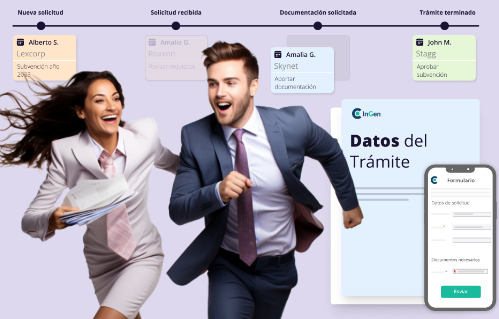
\includegraphics[width=0.7\textwidth]{assets/r2docuotimeline}
    \caption{Captura del homepage de R2 Docuo donde se puede ver el timeline de un trámite}{Fuente: https://www.r2docuo.com/es/expedientes-y-tramites}
    \label{fig:r2docuotimeline}
\end{figure}

Se debe notar que si bien los dos primeros logran la funcionalidad deseada en este proyecto, no permiten la personalización, no son necesariamente software libre y no se pueden introducir en sistemas más grandes de la misma manera que lo haría un paquete de software reutilizable.

\subsection{Paquetes de software que facilitan la creación de módulos de trámites}

La cantidad de paquetes de software que existen y que se puede considerar que ayudan en el proceso de gestión, control y seguimiento de trámites es abundante, por lo que nos centraremos en aquellas presentes en el ecosistema de \textit{Laravel}.

El seguimiento de trámites requiere que tengamos guardada la información de todos los pasos de un trámite y los cambios realizados. Además, la naturaleza de los trámites, como se podrá ver en el análisis de la solución, tiene que ver con estados (pasos de un procedimiento administrativo). Es por esto que las siguientes librerías podrían ser utilizadas con un objetivo similar al paquete que se pretende desarrollar en este proyecto:

\begin{itemize}
    \item \textit{Laravel Auditing}: Permite mantener control sobre los datos en una aplicación y para hacer seguimiento de los cambios realizados en los mismos. Es muy potente y fácil de usar.
    \item \textit{Laravel Eloquent State Machines}: Máquinas de estado aplicadas sobre los modelos \textit{Eloquent} (figura \ref{fig:laravelstatemachines}).
    \item \textit{Laravel-Permission}: Permite asociar usuarios con roles.
\end{itemize}

\begin{figure}[!htpb]
    \centering
    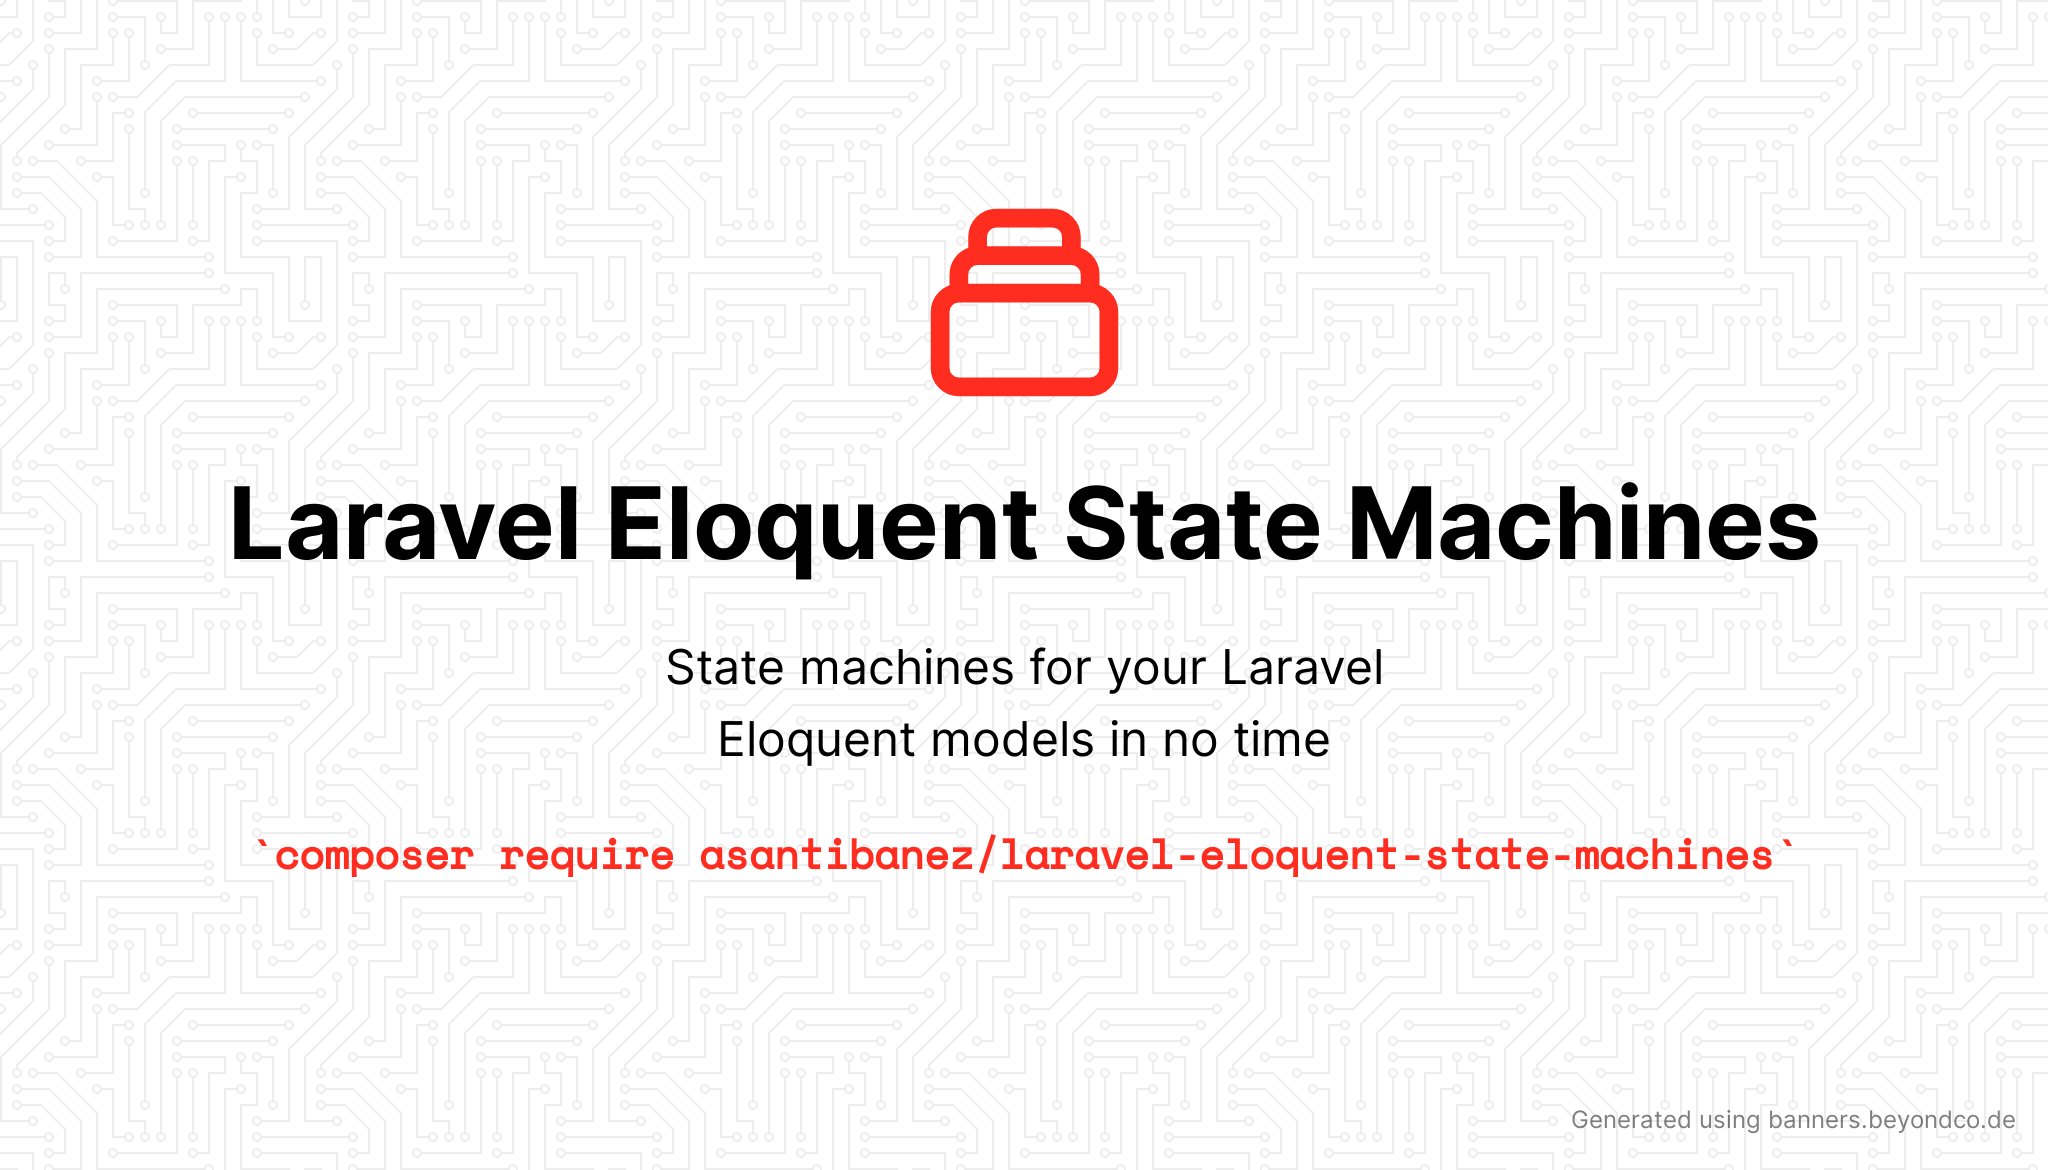
\includegraphics[width=0.7\textwidth]{assets/laravelstatemachines}
    \caption{Paquete de manejo de estados en Laravel}{Fuente: https://github.com/asantibanez/laravel-eloquent-state-machines}
    \label{fig:laravelstatemachines}
\end{figure}

De los tres paquetes anteriores, sin duda el de las máquinas de estados es el que más inspirará este proyecto. La funcionalidad es similar a la que se pretende, pero no es específica a los procesos administrativos y por lo tanto no brinda ciertas herramientas que podrían ser necesarias en los mismos, como el seguimiento, el cual podría ser implementado con la ayuda del segundo paquete mencionado.
